\documentclass{standalone}
\usepackage{fontspec}
\setsansfont{DejaVu Sans}
\usepackage{tikz}
\usetikzlibrary{arrows.meta}
\begin{document}
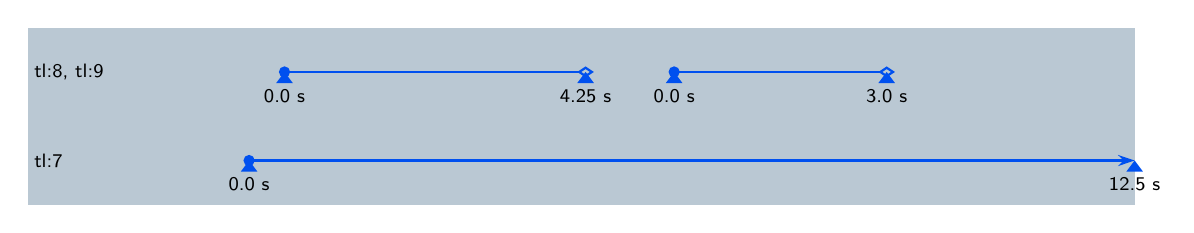
\begin{tikzpicture}[x=1pt,y=1pt,line width=0.8pt,inner sep=2pt,font=\sffamily\fontsize{7}{8.4}\selectfont]
\definecolor{ts000000}{HTML}{000000}
\definecolor{ts0050EF}{HTML}{0050EF}
\definecolor{tsBAC8D3}{HTML}{BAC8D3}
\fill[tsBAC8D3] (0,0) rectangle (400,64);
\draw[ts0050EF,{Circle[length=4pt]}-{Stealth[length=6pt,width=4pt,inset=2pt]},shorten <=-2pt] (80,16) -- (400,16);
\draw[ts0050EF,{Circle[length=4pt]}-{Diamond[open,length=6pt,width=4pt]},shorten <=-2pt,shorten >=-3pt] (92.8,48) -- (201.6,48);
\draw[ts0050EF,{Circle[length=4pt]}-{Diamond[open,length=6pt,width=4pt]},shorten <=-2pt,shorten >=-3pt] (233.6,48) -- (310.4,48);
\fill[ts0050EF] (80,16) -- (77,12) -- (83,12) -- cycle;
\fill[ts0050EF] (400,16) -- (397,12) -- (403,12) -- cycle;
\fill[ts0050EF] (92.8,48) -- (89.8,44) -- (95.8,44) -- cycle;
\fill[ts0050EF] (201.6,48) -- (198.6,44) -- (204.6,44) -- cycle;
\fill[ts0050EF] (233.6,48) -- (230.6,44) -- (236.6,44) -- cycle;
\fill[ts0050EF] (310.4,48) -- (307.4,44) -- (313.4,44) -- cycle;
\node[anchor=west,text=ts000000] at (0,48) {tl:8, tl:9};
\node[anchor=west,text=ts000000] at (0,16) {tl:7};
\node[anchor=north,text=ts000000] at (80,12) {0.0 s};
\node[anchor=north,text=ts000000] at (400,12) {12.5 s};
\node[anchor=north,text=ts000000] at (92.8,44) {0.0 s};
\node[anchor=north,text=ts000000] at (201.6,44) {4.25 s};
\node[anchor=north,text=ts000000] at (233.6,44) {0.0 s};
\node[anchor=north,text=ts000000] at (310.4,44) {3.0 s};
\end{tikzpicture}
\end{document}
